%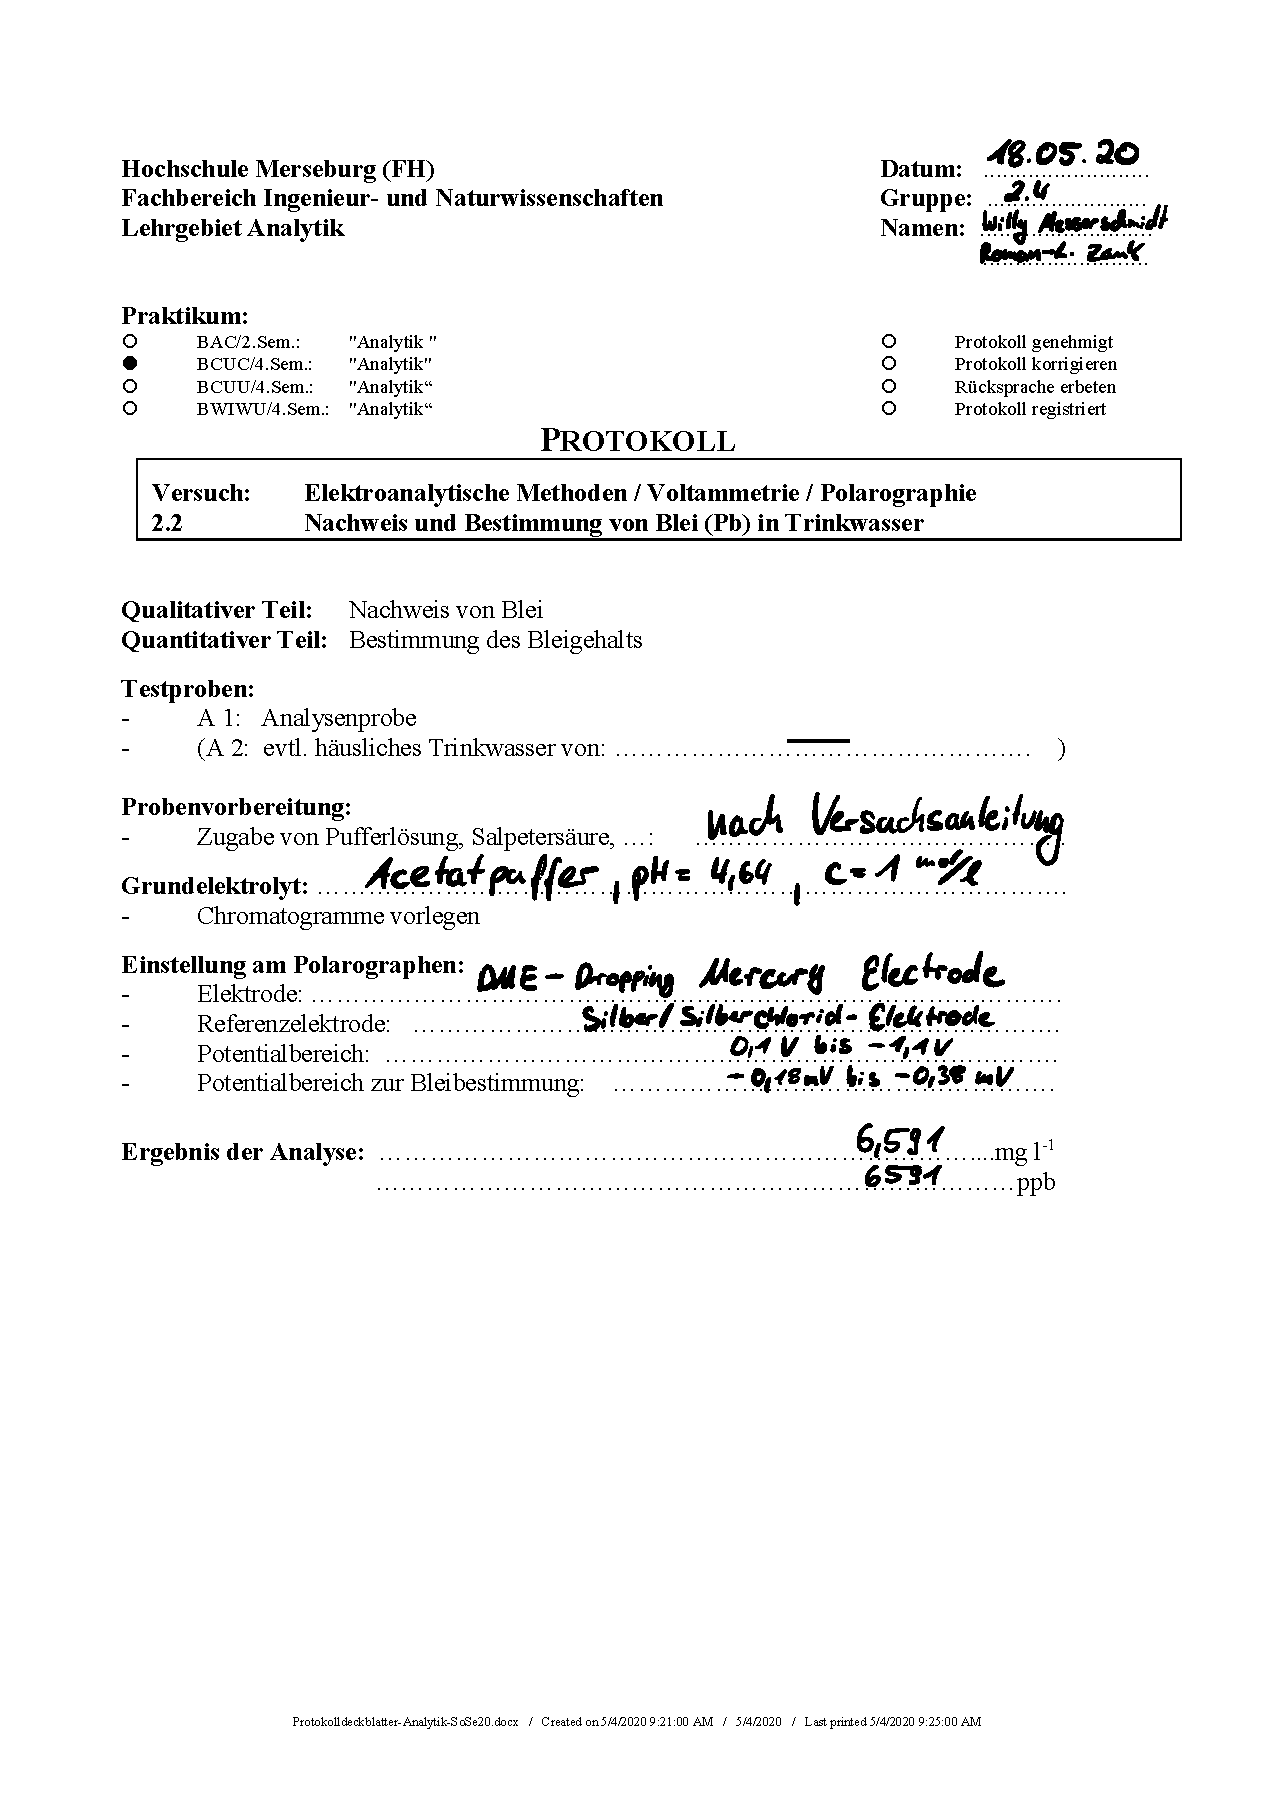
\includepdf[]{Deckblatt}
\pagebreak
\section{Einleitung}
\label{sec:einleitung}
Ein hoher Chloridgehalt im Trink-, sowie Brauchwasser kann aufgrund von Geschmacksbeeinträchtigung bei der Herstellung von Getränken wie Tee oder Kaffee unerwünscht sein. Für eisenhaltige Metalle können zu hohe Chloridgehalte sogar korrosiv wirken. Die Herkunft von erhöhten Chloridgehalten kann in Abwässern, Düngemitteln oder auch Fäkalien liegen. Unter der Voraussetzung, dass das Trinkwasser nicht korrosiv wirken sollte, gilt es, laut Trinkwasserverordnung, einen Grenzwert von \SI{250}{\milli \gram \per \liter} Chlorid einzuhalten.\\
Im Praktikum wird eine Leitungswasserprobe mittels Argentometrie auf diesen Grenzwert untersucht. Für die Titration werden die Messmethoden der Konduktometrie und Potentiometrie angewandt. Im Protokoll sind dabei verschiedene Methoden für Äquivalenzpunktbestimmung darzustellen. 




